\section{Limitations of Orchestration Decidability}

\mnote{Different approaches to achieve optimality}
We introduced the orchestration problem as the problem to find a consistent orchestration if it exists.
This is equivalent the existence of an optimal orchestration function.
We can distinguish two approaches to ensure that the orchestration function is optimal, i.e., that it does always find a consistent orchestration if it exists.
Let $P$ be the problem space, i.e., all possible transformation execution orders for given transformations and let $S_{i}$ be the solution space with those orders that yield consistent models for a specific input of models and a change to them.
\begin{properdescription}
    \item[Strategy Definition:] Define a strategy that explores the problem space $P$ to find one of the sequences in the solution space $S_{i}$, if $S_{i} \neq \emptyset$.
    \item[Transformation Restriction:] Define a \emph{well-behavedness} property for the transformations that ensures that executing the transformations in any order often enough, they yield consistent models if $S_{i} \neq \emptyset$, i.e., for any given input $i$ there is an $n \in \mathbb{N}$ such that $\forall s \in P : \abs{s} > n \Rightarrow s \in S_{i}$.
\end{properdescription}

%Unfortunately, optimality is a property that we cannot request from an orchestration function. Optimality would mean that the orchestration function can decide whether there is sequence of transformations that leads to consistent models and thus terminate.

\mnote{No restrictions to transformations}
In the latter case, the orchestration function may return any order of the transformations, as long as the sequence is long enough to be optimal.
This means, performing an iterative execution of the transformations leads to a consistent result, comparable to a fixed-point iteration.
Since optimality is a property of an orchestration function with respect to a set of transformations, defining a \emph{well-behavedness} property as a restriction for transformations to ease finding an optimal orchestration function will potentially not concern a single transformation but the set of them.
This can easily contradict our assumption of independent development and reuse or lead to restrictions of transformation that are not practical anymore.

\mnote{Section summary}
In the following, we first investigate the possibility to find an optimal orchestration function without restricting the transformations.
We define a general algorithm that realizes an application function, as in practice the function will be realized in terms of an algorithm that dynamically selects the next transformation to execute rather than being an ordinary mathematical function.
We then discuss its correctness and termination and relate it to the orchestration problem.
After proving undecidability of the orchestration problem, we discuss the possibilities to restrict transformations such that the problem get decidable.
Finally, we shortly discuss confluence as a considerable property of transformation networks.

% Thus, we first follow the former approach and investigate the possibility to find an optimal orchestration function without restricting the transformations.
% %Optimality of an orchestration function means that it can decide whether there is a sequence of transformations that leads to consistent models and thus terminates.
% In the following, we therefore define a general algorithm that realizes an application function and investigate how we can ensure that its orchestration function is optimal.


\subsection{An Algorithm for the Application Function}

%Start with defining an algorithm that realizes the application function. (different options depending on when to return $\bot$, discussed later)
%First option: we assume an oracle that returns the transformation to execute next according to the orchestration function and we stop when consistent models are achieved

%\todo{Transformations as variable instead of index and say that our implementation will be independent from concrete network. But in general, once could define it specific for a set of transformations.}
%\todo{Rename generatedChanges and executedTransformation to $\change{generated}$ and new command transformationtuple with index executed}
\newcommand{\applyalgexecuted}{\sequence{\transformation{t}_{\mathvariable{executed}}}}
\newcommand{\applyalggenerated}{\sequence{\changetuple{\metamodeltuple{M}, \mathvariable{generated}}}}
\begin{algorithm}
   % \begin{algorithmic}[1]
    \Procedure{\function{FindCorresponding}}{$\consistencyrelation{CR}{}, \conditionelement{c}{l}, \model{m}{2}, \model{m}{\mathvariable{traces}}$}
        \algindentskip
        \State $\mathvariable{tracedElements} \gets \setted{\conditionelement{c}{r} \mid \tupled{\conditionelement{c}{l}, \conditionelement{c}{r}} \in \model{m}{\mathvariable{traces}}}$
        \For{$\conditionelement{c}{r} \in \mathvariable{tracedElements}$} \label{algo:synchronization:find_corresponding_elements:line:explicit}
            \If{$\tupled{\conditionelement{c}{l}, \conditionelement{c}{r}} \in \consistencyrelation{CR}{}$}
                \State \Return{$\conditionelement{c}{r}$}
            \EndIf
        \EndFor
        \algblockskip

        \For{$\conditionelement{c}{r} \in \mathcal{P}(\model{m}{2})$} \label{algo:synchronization:find_corresponding_elements:line:implicit}
            \If{$\tupled{\conditionelement{c}{l}, \conditionelement{c}{r}} \in \consistencyrelation{CR}{}$}
                \State $\model{m}{\mathvariable{traces}} \gets \model{m}{\mathvariable{traces}} \cup \setted{\tupled{\conditionelement{c}{l},\conditionelement{c}{r}}}$
                \State \Return{$\conditionelement{c}{r}$}
            \EndIf 
        \EndFor
        \algblockskip

        \State \Return{$\bot$}
        \algindentskip
    \EndProcedure
\end{algorithmic}
    \begin{algorithmic}[1]
        \Procedure{$\function{Apply}$}{$\transformationset{T}, 
        \modeltuple{m} %= \tupled{\model{m}{1}, \dots, \model{m}{n}}
        , \changetuple{\metamodeltuple{M}} %= \tupled{\change{\metamodel{M}{1}}, \dots, \change{\metamodel{M}{n}}}
        $}
            \State $\mathvariable{isConsistent}$ $\leftarrow$ $\function{CheckConsistency}(\transformationset{T}, \modeltuple{m})$
            \If{$\neg \mathvariable{isConsistent}$}
                \State \Return{$\bot$}
            \EndIf
            \State $\applyalgexecuted \leftarrow \sequenced{}$
            \State $\applyalggenerated \leftarrow \sequenced{}$
            \State $\transformation{t}_{next}$ $\leftarrow$ $\function{Orchestrate}_{\transformationset{T}}(\modeltuple{m}, \changetuple{\metamodeltuple{M}}, \applyalgexecuted, \applyalggenerated)$ \label{algo:orchestration:application:line:startorchestrate}
            \While{$\transformation{t}_{next} \neq \bot$}
                \State $(\modeltuple{m}, \changetuple{\metamodeltuple{M}})$ $\leftarrow$ $\generalizationfunction{\metamodeltuple{M}, \transformation{t}_{next}}(\modeltuple{m}, \changetuple{\metamodeltuple{M}})$ \label{algo:orchestration:application:line:stepcalculation}
                \State $\applyalgexecuted \gets \applyalgexecuted + \transformation{t}_{next}$
                \State $\applyalggenerated \gets \applyalggenerated + \changetuple{\metamodeltuple{M}})$
                \State $\transformation{t}_{next}$ $\leftarrow$ $\function{Orchestrate}_{\transformationset{T}}(\modeltuple{m}, \changetuple{\metamodeltuple{M}}, \applyalgexecuted, \applyalggenerated)$
            \EndWhile \label{algo:orchestration:application:line:endorchestrate}
            %\State $\tupled{\model{m}{1}, \dots, \model{m}{n}} \leftarrow \modeltuple{m}$
            %\State $\tupled{\change{\metamodel{M}{1}}, \dots, \change{\metamodel{M}{n}}} \leftarrow \changetuple{\metamodeltuple{M}}$
            \State $\modeltuple{m}_{res} \leftarrow \changetuple{\metamodeltuple{M}}(\metamodeltuple{m})$ %\tupled{\change{\metamodel{M}{1}}(\model{m}{1}), \dots, \change{\metamodel{M}{n}}(\model{m}{n})}$
            \State $\mathvariable{isConsistent}$ $\leftarrow$ $\function{CheckConsistency}(\transformationset{T}, \modeltuple{m}_{res})$ \label{algo:orchestration:application:line:startconsistencycheck}
            \If{$\neq \mathvariable{isConsistent}$}
                \State \Return{$\bot$}
            \EndIf \label{algo:orchestration:application:line:endconsistencycheck}
            % \For{$\transformation{t} \in \transformationset{T}$} \label{algo:orchestration:application:line:startcheckconsistency}
            %     %\State $(\consistencyrelation{CR}{}, \consistencypreservationrule{\consistencyrelation{CR}{}}) \leftarrow \transformation{t}$
            %     \State $\mathvariable{isConsistent}$ $\leftarrow$ $\function{CheckConsistency}_{\metamodeltuple{M}}(\modeltuple{m}_{res}, \transformation{t}$) %\consistencyrelation{CR}{})$
            %     \If{$\neq \mathvariable{isConsistent}$}
            %         \State \Return{$\bot$}
            %     \EndIf
            % \EndFor \label{algo:orchestration:application:line:endcheckconsistency}
            \State \Return{$\modeltuple{m}_{res}$} \label{algo:orchestration:application:line:returnresult}
        \EndProcedure
    \end{algorithmic}
    \caption[Application function implementation]{Application function implementation.}
    \label{algo:orchestration:application}
\end{algorithm}

\mnote{Algorithm for the application function}
We have yet discussed the orchestration and application functions as purely mathematical functions.
In practice, however, they need to be implemented in terms of algorithms.
In \autoref{algo:orchestration:application}, we propose an algorithm for the application function.
It also encodes the orchestration function, because in contrast to the mathematical definition, an algorithm for the orchestration function will not determine a complete sequence of transformations for given models and changes, but dynamically select the next transformation to execute.
As soon as all transformation delivered by the orchestration are executed, it returns the resulting models if they are consistent or otherwise returns $\bot$.

\mnote{Algorithm is independent from concrete transformations}
An application function according to \autoref{def:applicationfunction} is parametrized by an orchestration function, which, in turn, is parametrized by the set of transformations $\transformationset{T}$ that it is supposed to be executed on.
A transformation network according to \autoref{def:transformationnetwork} is defined to consist of a set of transformations and an application function, which may suggest that both the application as well as the orchestration function can be defined specific for one network.
\autoref{algo:orchestration:application} reflects this by assuming an \function{Orchestrate} function that is specific for a set of transformations.
It may, however, be implemented by a generic function that works independent from the concrete transformations and, instead, accepts them as a parameter.
We do, however, focus on a general algorithm and \function{Orchestrate} that can be applied to any set of transformations.
In that case, the algorithm does not realize a single application function, but actually a family of application functions for all possible transformation sets $\transformationset{T}$.

\mnote{Algorithm dynamically selects next transformation}
The dynamic selection of transformations is realized by an \function{Orchestrate} function and stops as soon as no further transformations to apply are delivered.
The latter may be the case because the models are already consistent or because no further transformations can be applied.
It is essential that \function{Orchestrate} does only return a transformation that can be applied to the models and current changes, because otherwise its application by the $\generalizationfunction{}$ in Line~\ref{algo:orchestration:application:line:stepcalculation} would fail.
The complete logic of the orchestration function is combined with the application of the delivered sequence in Lines~\ref{algo:orchestration:application:line:startorchestrate}--\ref{algo:orchestration:application:line:endorchestrate}.
Since, in practice, the selection of transformation has to be performed dynamically anyway, an implementation of the orchestration function always needs to apply the transformations.
Thus a separation of the orchestration function into a separate algorithm, which performs the same steps as in Lines~\ref{algo:orchestration:application:line:startorchestrate}--\ref{algo:orchestration:application:line:endorchestrate} leads to a redundancy by applying the transformations both in the separate orchestration algorithm as well as in the given algorithm.

\mnote{Orchestration needs history of changes and transformations}
The function receives the history of executed transformations and generated changes, because if the complete orchestration function was implemented in a separate method, it would also be able to use that information to determine a proper orchestration.
Otherwise, its expressiveness would be restricted with respect to the definition of an orchestration function, because that function makes a global decision for all transformations to execute base on the original input, which is not available for the \function{Orchestrate} function after its first execution anymore.
In a practical implementation of that function, the history may, however, not be considered or truncated, depending on the information necessary for the concrete implemented orchestration strategy.

\mnote{Strategies for selecting next transformation}
%The \function{Orchestrate} function is responsible for selecting the next transformation.
The \function{Orchestrate} function may implement different strategies, which we will later discuss in more detail.
The most simple strategy would be to execute the same order of transformations iteratively, thus always executing that transformation who was not executed for the longest time.
Another reasonable strategy would be to manage a queue of transformation and after executing one transformation to enqueue all transformations that are adjacent to the metamodels of the two models that were modified by the transformation if they are not yet enqueued.
This ensures that those transformation are executed next which can process changes that have just been produced by another transformation.
Both these strategies are independent from the concrete transformations and could thus be implemented in a function that can be used for any set of transformations $\transformationset{T}$.
In \autoref{chap:orchestration:algorithm}, we will discuss a specific orchestration strategy.
Until then, the concrete strategy is not important and any of the exemplified ones can be imagined.

\mnote{Assumed further functions of algorithm}
Next to \function{Orchestrate}, the algorithm uses the external functions $\generalizationfunction{}$ and \function{CheckConsistency}.
The $\generalizationfunction{}$ function is the generalization function, which simply applies the given transformation to the appropriate models of the given tuple.
The \function{CheckConsistency} checks whether the given models are consistent to the set of transformations, according to \autoref{def:consistencytransformation}.
This function can be implemented in two ways.
First, it may be implemented as an explicit check regarding the consistency relations of the transformations.
If the transformations are defined by their consistency relations, from which a transformations language derives the consistency preservation rules, such as \gls{QVTR}, the models can be checked regarding the given relations.
In case of \gls{QVTR}, the transformations can be executed in \emph{checkonly mode}~\cite[Sec. 7.9]{qvt}.
Second, it may be implemented by (virtually) executing the consistency preservation rule and checking whether its execution performed changes.
If the transformations are hippocratic, i.e., if they do not perform changes when the models are already consistent, this way consistency can be checked.
This is always necessary when the consistency relations are not explicitly given but implicitly defined as the image of the consistency preservation rules, such as for transformation defined in \gls{QVTO}.
Due to their simplicity, we do not provide an explicit implementation of these two functions.

% Algorithm dynamically selects next transformation.
% It stops as soon as orchestration does provide further transformations.
% Then, either no transformation can be applied anymore, or the models are consistent.
% This moves some of the logic of the orchestration function into the apply function, as orchestrate only selects the next function rather than delivering a sequence in the beginning.
% Thus, Lines~\ref{algo:orchestration:application:line:startorchestrate}--\ref{algo:orchestration:application:line:endorchestrate} implement the orchestration function.
% This is reasonable for two reasons:
% First, this is how a practical algorithm will perform the selection anyway, by dynamically selecting the next transformation.
% Second, this is only a matter of implementation, as we could move the lines to a separate method, which acts as the orchestrate function by determining the sequence by dynamically applying the transformations, let it return the sequence and then let the apply function apply the transformations in that order again.
% %Second, although dynamic selection may sound more expressive than a a priori determination of the complete sequence like defined for the app and orc function in the previous definitions, this is not the case as an orc function according to that definition may be an oracle that, in a practical implementation, determines the sequence for a given input in the same way.
% Since applying the transformation in the orc function to determine a sequence and then simply applying them in the app function again is redundant, we directly implemented that dynamic selection in the app function.

% Apply is defined to be comprehensible, not efficient. For example, the consistency check can be improved by aborting as soon as one transformation to which the models are inconsistent is found.

% Gen is the generalization function, CheckConsistency is generalized consistency checker which just checks for the appropriate models in the tuple.

%\todo{transformation set should be parameter, not one application/orchestration function per transformation set}


\subsection{Correctness and Termination of the Algorithm}
\label{chap:orchestration:decidability:correctness_termination}

\mnote{Algorithms implements correct application function}
\autoref{algo:orchestration:application} is constructed to implement an application function according to \autoref{def:applicationfunction}.
It is designed to be correct, i.e., it only returns models when they are consistent.
We show that the algorithm fulfills these properties in the following theorem.

\begin{theorem}[Apply Algorithm Correctness]
    The \function{Apply} function in \autoref{algo:orchestration:application} fulfills the functional behavior of an application function as defined in \autoref{def:applicationfunction} and is correct according to \autoref{def:applicationfunctioncorrectness}
\end{theorem}
\begin{proof}
    The \function{Apply} function fulfills the input and output requirements of an application function according to \autoref{def:applicationfunction}.
    It only returns a model tuple in Line \ref{algo:orchestration:application:line:returnresult}, which is achieved by applying the changes delivered by the sequence of transformations delivered by the orchestration function realized as a repeated call of the \function{Orchestrate} function in Lines~\ref{algo:orchestration:application:line:startorchestrate}--\ref{algo:orchestration:application:line:endorchestrate}.
    Thus, \function{Apply} fulfills the definition of an application function.

    Correctness of an application function according to \autoref{def:applicationfunctioncorrectness} requires the output models, if not returning $\bot$, to be consistent to the consistency relations of all transformations, as long as the input models were consistent.
    The algorithm only returns models in \autoref{algo:orchestration:application:line:returnresult}.
    These models are always consistent to the consistency relations of all transformations, because Lines~\ref{algo:orchestration:application:line:startconsistencycheck}--\ref{algo:orchestration:application:line:endconsistencycheck} ensure this and otherwise return $\bot$ before.
\end{proof}

\mnote{Termination is not guaranteed}
In addition to being correct, the algorithm needs to terminate always.
Non-termination can only occur because of the loop for orchestration transformations, as there are no recursions and the other loop is finite because the set of transformations is of finite size.
According to the definition, an orchestration function is defined to return a finite sequence of transformations, which would also result in a finite number of execution of the loop for orchestrating transformations.
The implementation by a dynamic selection of the next transformation to execute can, however, lead to an infinite sequence of transformations.
The \function{Orchestrate} function receives the list of previously executed transformations, as otherwise it would never be able to identify that, for example, always the same sequence of transformations is executed and leads to the same changes, thus the algorithms is only performing an infinite alternation.
We do, however, need to ensure that the \function{Orchestrate} function returns $\bot$ after a finite number of calls.

\mnote{Options to guarantee termination}
If we assume that we can achieve optimality for the orchestration function, we would have the guarantee that if a consistent orchestration exists, the function will find it.
There is, however, no restriction to what the orchestration function may return when there is no orchestration that yields consistent models at all.
Thus, we have two options to ensure termination:
\begin{properenumerate}
    \item We enable the orchestration function to identify whether a consistent orchestration exists.
    \item We find an upper bound for the number of necessary transformation executions, such that if more transformations were executed, we cannot expect the algorithm to find consistent models anymore and thus abort. 
\end{properenumerate}

\mnote{Termination and optimality are conflicting}
The simplest solution would be to find an upper bound for the number of necessary transformation executions.
We will, however, prove in the following that there is no such upper bound.
Afterwards, we will show that identifying whether a consistent orchestration exists is not possible either.
This will lead to the insight that we cannot guarantee termination of the algorithm with an optimal orchestration function.


%\subsection{Upper Execution Bound}

\mnote{No general upper bound for necessary number of executions}
With the example in \autoref{fig:orchestration:necessity_multiple_executions}, in which values are incremented by one upon each execution of one specific transformation until a fixed but arbitrary value $x$ is reached, we were able to show in \autoref{lemma:minimal_executions} that there can be transformation networks in which a transformation needs to be executed at least $x-1$ times for a fixed but arbitrary $x$ until consistent models are models.
Thus, any consistent orchestration contains that transformation at least $x-1$ times.
While we have used that to show that executing each transformation only once is, in general, not sufficient, we can also easily show the more general statement that we cannot find a maximal length for the orchestration of transformation networks of specific size.

\begin{theorem}[Upper Bound for Shortest Consistent Orchestration]
    \label{theorem:orchestration_fixed}
    For every $n$, there is a set of transformations $\transformationset{T}$ such that for specific models $\modeltuple{m}$ and changes $\changetuple{}$ to them for which each possible orchestration function $\orcfunction{\transformationset{T}}$ with whom $\appfunction{\orcfunction{\transformationset{T}}}(\modeltuple{m}, \changetuple{})$ is consistent, delivers a sequence as $\orcfunction{\transformationset{T}}(\modeltuple{m}, \changetuple{})$ with $\abs{\orcfunction{\transformationset{T}}(\modeltuple{m}, \changetuple{})} > n$.
\end{theorem}
\begin{proof}
    We know from \autoref{lemma:minimal_executions} that $\transformationset{T}_{inc}$ requires at least $x-1$ executions of $\transformation{t}_{12}$ for the inputs defined in \autoref{lemma:minimal_executions} and the fixed but arbitrary value $x$.
    Thus, with $x \geq n+2$ for $\transformationset{T}_{inc}$, we know that at least $x-1 = n+1$ executions of $\transformation{t}_{12}$ are necessary.
    Let $\modeltuple{m}$ and $\changetuple{}$ be the inputs defined in \autoref{lemma:minimal_executions}.
    Then for any orchestration function $\orcfunction{\transformationset{T}}$ that delivers a consistent orchestration for these inputs, we know that $\abs{\orcfunction{\transformationset{T}}(\modeltuple{m}, \changetuple{})} >= x-1 = n+1 > n$.
    This proves the theorem by example.
\end{proof}

\mnote{Upper bound cannot be used to decide whether consistent orchestration exists}
In consequence, it is not possible to find a fixed value or a value only depending on the transformation network size that defines an upper bound for the necessary number of transformation executions to yield consistent models, i.e., there is no upper bound for the shortest consistent orchestration.
Thus, even if we are able to ensure optimality of orchestration with the \function{Apply} and \function{Orchestrate} functions, there is no upper bound for the number of transformation execution that is necessary for a consistent orchestration.
We cannot abort the execution after a fixed number of loop iterations without the possibility that consistent models would have been found if the execution had proceeded and thus not ensuring optimality.

%To avoid non-termination of the algorithm, we thus need to be able to ensure that the \function{Orchestrate} function at some point returns $\bot$.
%This means that it must be able to identify when no orchestration that yields consistent models exists at all, and if it exists it must be able to find it.

%Requirement: Know whether orchestration exists, otherwise impossible to find sequence always if it exists, as we do not know whether it exists.

% This is due to the reason that the \function{Orchestrate} function does only receive the current models and changes but not the history of executed transformations.
% Thus, it cannot identify which and how many transformation have already been executed and whether the current changes have already been produced before such that 

% There are, however, still derivations of the stepwise orchestrate to the original orchestration function:
% The stepwise application of the orchestrate function cannot derive a complete sequence but only make a local decision based on the given models and changes. Thus, if the transformations produce the same changes repeatedly, i.e., there is an alternation in the produced changes, the orchestrate function cannot detect that and always determinates the same sequences of transformations to be executed next. This results in an infinite sequence of execute transformations, which is conforming to the orchestration function definition, but still is a result of the possibilities of an actual and reasonable implementation of that function.
%Additionally, the function may be able to determine beforehand whether an orchestration that yields consistent models exists and otherwise return $\bot$ in its first application.
%A practical implementation, however, will not act that way but instead determine the next transformation until no transformation can be applied anymore.
%In consequence, it is possible that several transformations are executed before detecting that no orchestration can be found.
%Since the orchestration is encoded in the apply function anyway and the function then still returns $\bot$, this is not a problem.
%This affects termination.

%Algorithm is correct if it returns only consistent models. Additionally, it must always terminate.
%ADD DEFINITION!

%Correctness is given by construction and easy to achieve.
%Termination if no transformation can be applied or consistent models are found.

%Thus: We need to find an order of transformation such that the result is consistent.

%Give example, where no execution order exists that terminates. Thus, the algorithm does not terminate.

%Approach: We want to decide whether an order exists or not.


\subsection{Undecidability of the Orchestration Problem} %Undecidability of Orchestration}

\mnote{Impossible to decide whether consistent orchestration exists}
To ensure termination of the \function{Apply} algorithm with an optimal orchestration function, we need to identify the case that no consistent orchestration exists, because that is the only situation in which otherwise an infinite number of transformation execution is possible.
Unfortunately, we will show that the problem to decide whether such an orchestration exists or not is undecidable.
To do so, we reduce the halting problem for Turing machines to the orchestration problem.
Thus, solving the orchestration problem would solve the halting problem.
We have published a simplified version of this proof, based on a more concise modelling formalism, in \cite{gleitze2020orchestration}.

\begin{figure}
    \centering
    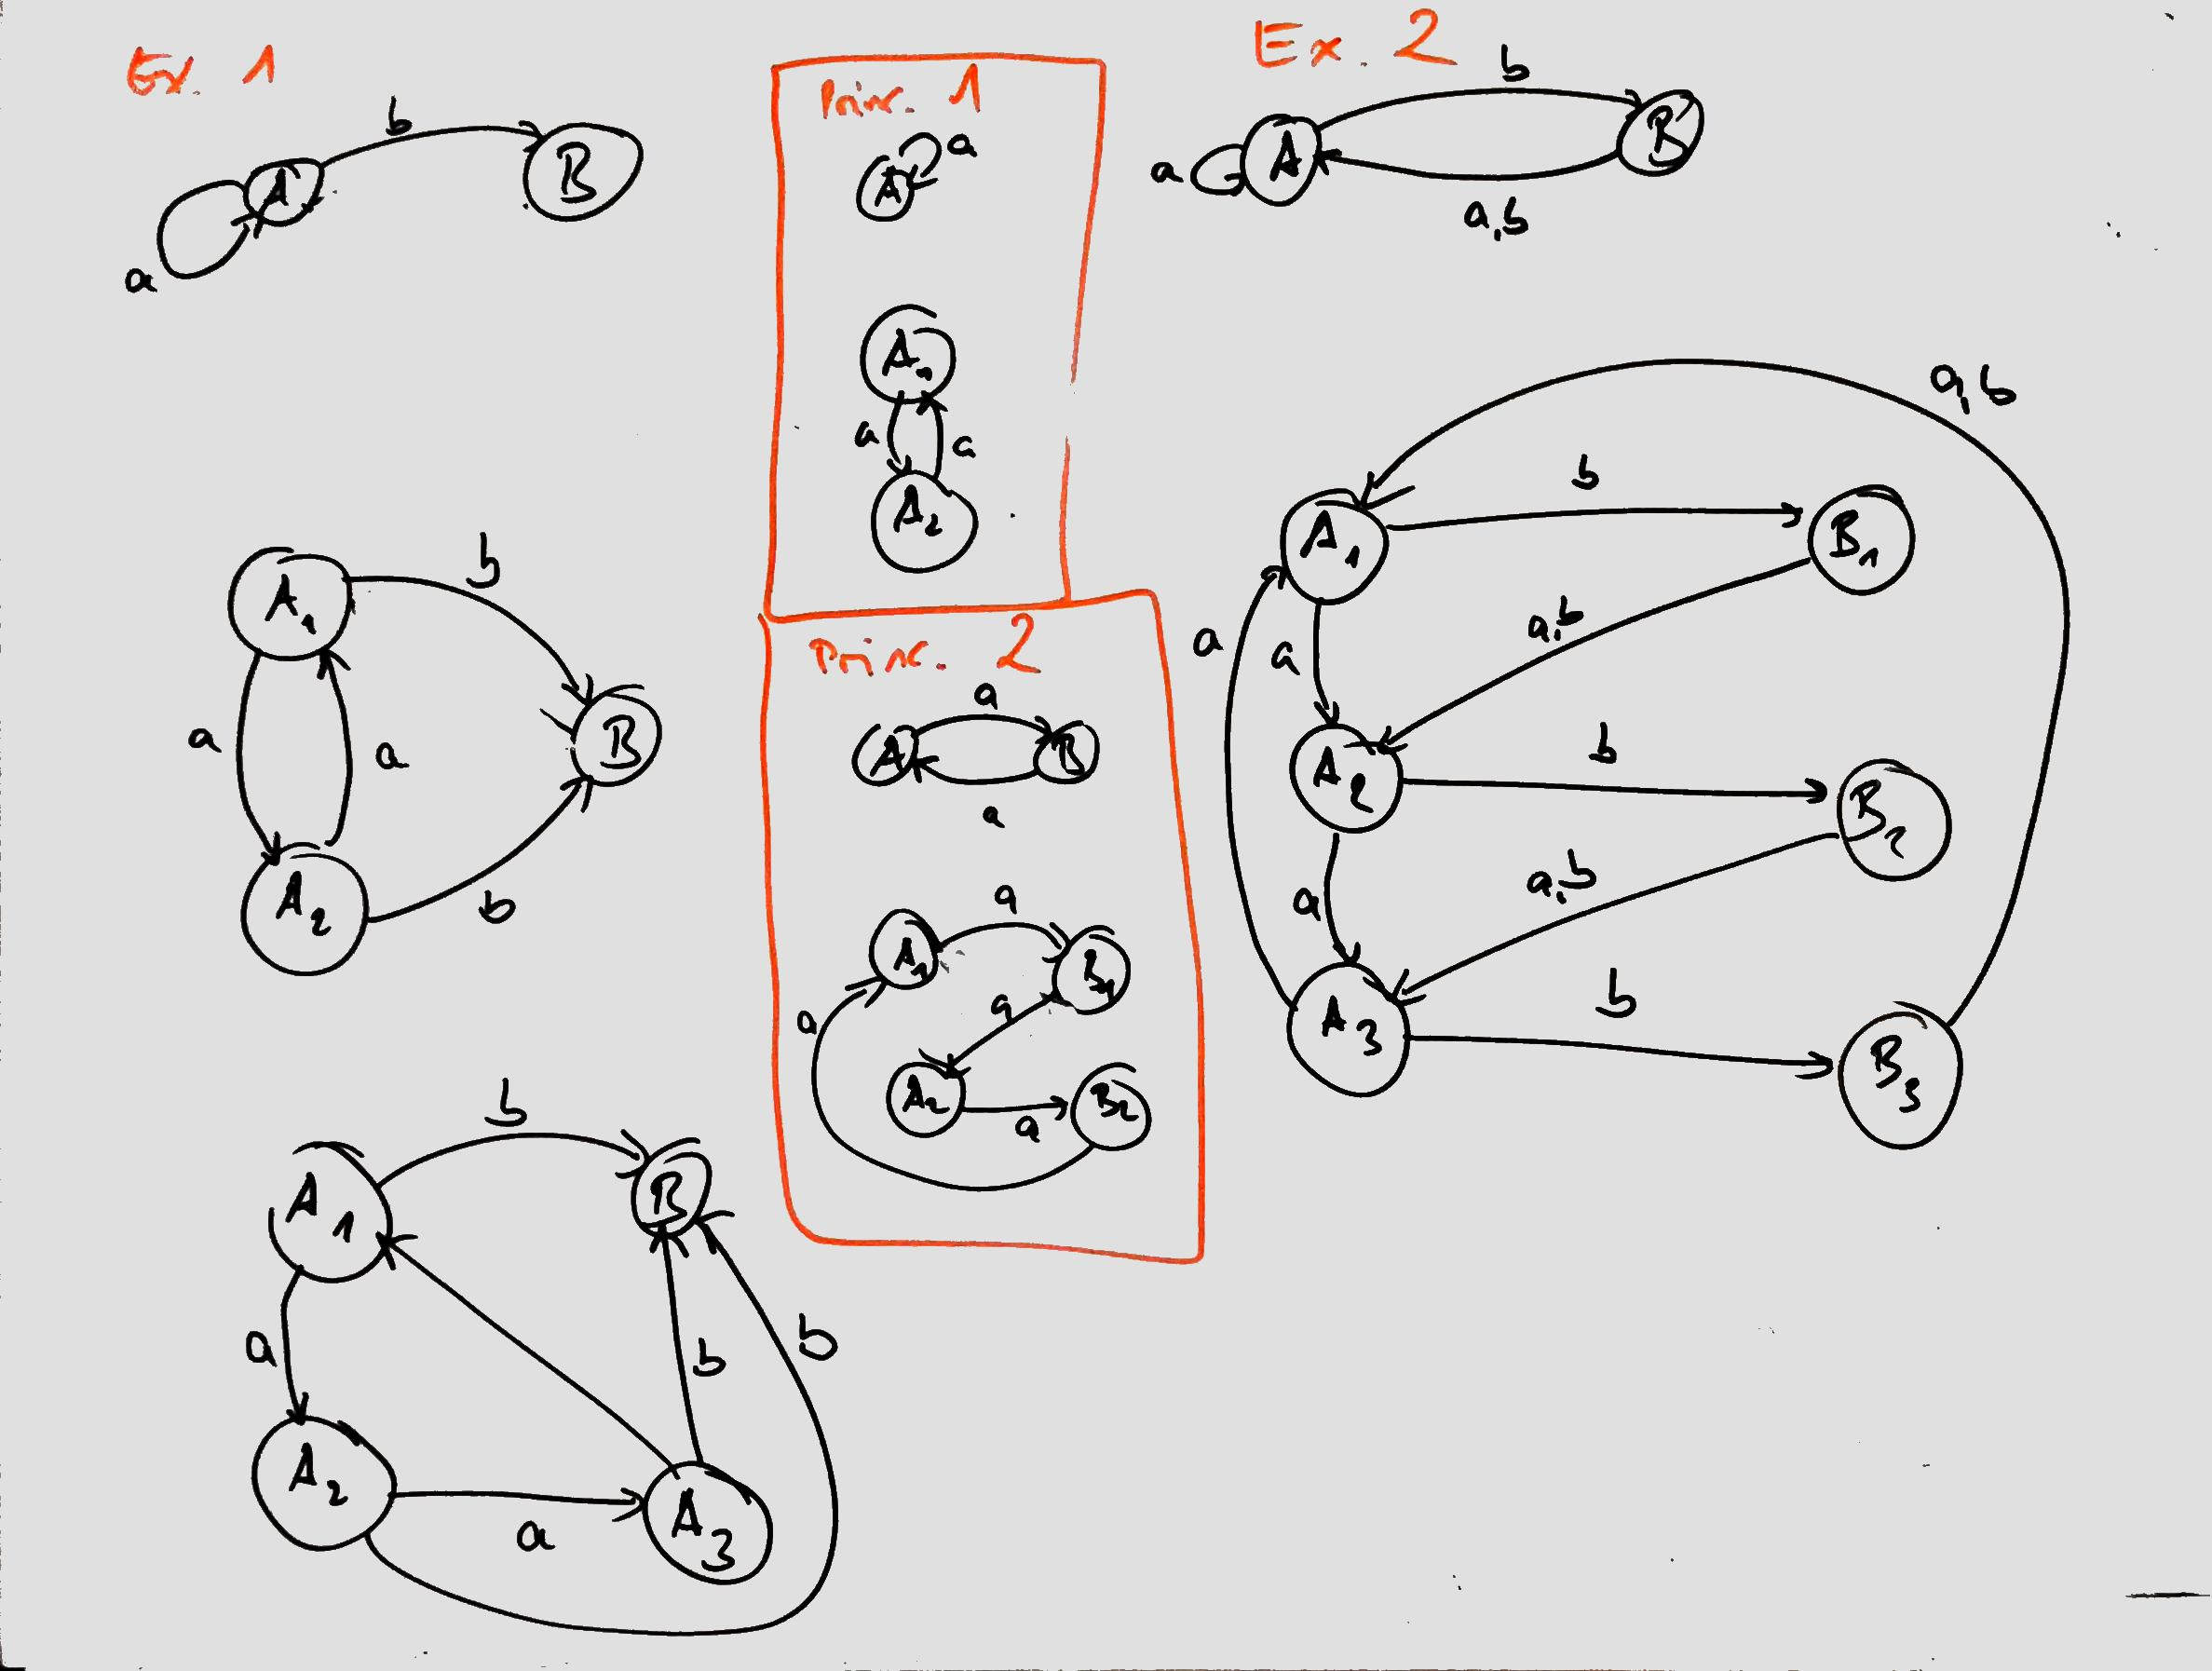
\includegraphics[width=0.9\textwidth]{figures/correctness/orchestration/cycle_elimination.jpg}\\
    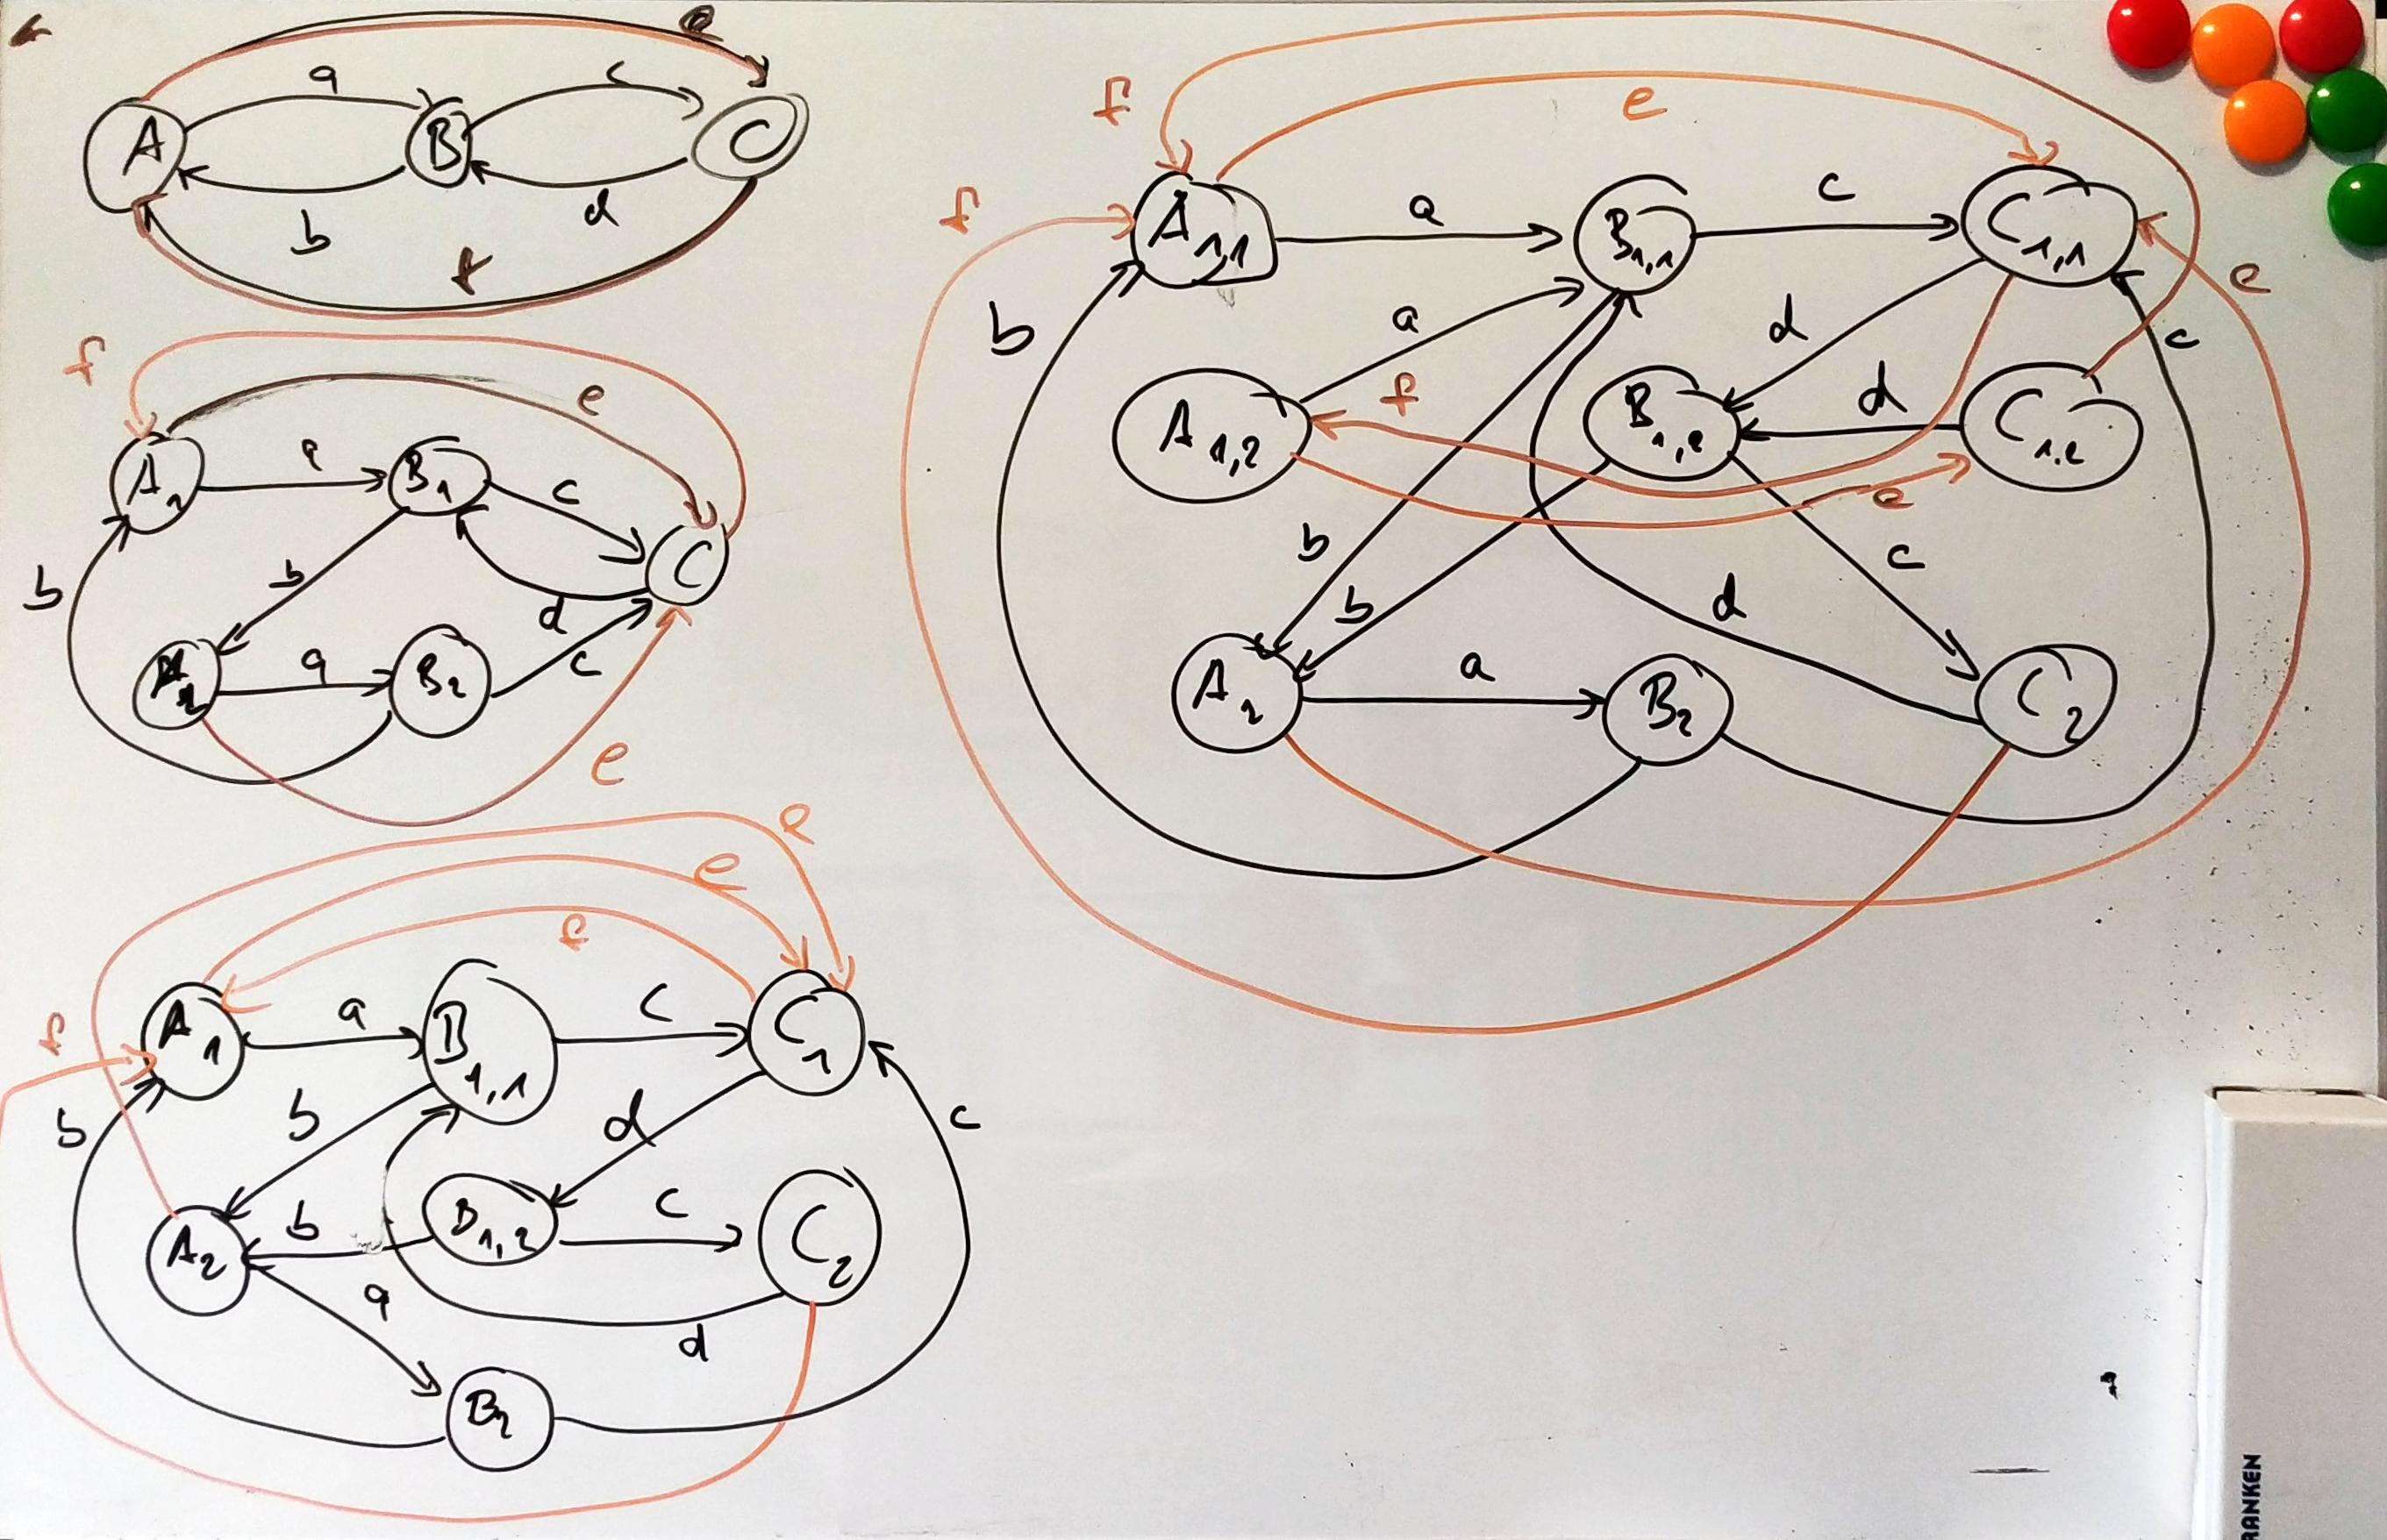
\includegraphics[width=0.9\textwidth]{figures/correctness/orchestration/cycle_elimination2.jpg}
    \caption[Cycle elimination in Turing machine transition functions]{Principles to eliminate cycles of length $\leq 2$ in transition function of a Turing machine and two application examples.}
    \label{fig:orchestration:cycle_elimination}
\end{figure}

\mnote{Assumptions for Turing machine}
Given a Turing machine $\TuringMachine$ over some alphabet $\Sigma$, we construct metamodels $\metamodeltuple{M}_{\TuringMachine}$ and a transformation network with a set of transformations $\transformationset{T}_{\TuringMachine}$, as well as initial models $\modeltuple{m}_{\TuringMachine, x} \in \metamodeltupleinstanceset{M_{\TuringMachine}}$ and changes $\changetuple{\metamodeltuple{M},\TuringMachine,x}$ for them for which a consistent orchestration exists if, and only if, $\TuringMachine$ halts on input $x \in \Sigma^*$.
Without loss of generality, we assume that the graph of the transition function of $\TuringMachine$ contains no cycles of length $\leq 2$.
This means that does not contain no self-loops, i.e., that the transition function always changes the state.
And that there is no cycle between two states.
This is without loss of generality, because cycles of these two lengths can be eliminated by duplicating states.
A self-loop can be eliminated by duplicating the state with a cycle of length $2$ between the duplicated states,  replicating all outgoing transitions for both states and let all ingoing transitions go to one of these two states.
Likewise, eliminating cycles of length $2$ can be achieved by duplicating both involved states and replacing the cycle of length $2$ by one of length $4$, replicating all outgoing transitions for all states and let all ingoing transitions go to one of the two states of each replicated one.
Inductively applying these duplication principles can eliminate all cycles of length $\leq 2$.
The two principles and the application to a scenario with self-loops as well as three states with pairwise cycles of length $2$ are depicted in \autoref{fig:orchestration:cycle_elimination}.

\mnote{Models representing states of Turing machine}
We construct models that consist of a timestamp, the tape content and the tape position.
With our formalism, we can, for example, encode this into a metamodel $\metamodel{M}{\TuringMachine}$ having one class with exactly these contents and models that do only contain one instance of that class.
For reasons of simplicity, we do not explicitly denote the according metamodel and denote a model $\model{m}{}$ as $\model{m}{} \in \mathbb{N}_0 \times \Sigma^* \times \mathbb{N}_0$.
We use one model for each state of the Turing machine and one transformation between each pair whose states have a transition between them.
To be able to identify the state which a model represents by its metamodel, we also assume one metamodel for each of the states, although they all look equal. Thus, we have $\metamodeltuple{M}_\TuringMachine = \tupled{\metamodel{M}{1, \TuringMachine}, \dots, \metamodel{M}{n, \TuringMachine}}$ with $n = \abs{Q_\TuringMachine}$ if we assume $Q_\TuringMachine = \setted{q_1, \dots, q_n}$ to be the set of states of $\TuringMachine$.
%Equivalently, we may also define $\abs{Q_\TuringMachine}$ metamodels with the same contents.
We define the following function that returns the state of the Turing machine represented by a metamodel:
\begin{align*}
     \function{Q} : %\setted{\metamodel{1,\TuringMachine}, \dots, \metamodel{n,\TuringMachine}} \rightarrow Q_\TuringMachine \\
     \metamodel{M}{i,\TuringMachine} & \mapsto q_i %\mathtext{with} \exists i \in \setted{1, \dots, n} : \model{m}{} \in \metamodelinstanceset{M}{i, \TuringMachine} \land q = q_i
\end{align*}
% We define the following function that returns the state of the Turing machine represented by a model:
% \begin{align*}
%      \function{Q} : \bigcup_{1 \leq i < n} \metamodelinstanceset{M}{i, \TuringMachine} & \rightarrow Q_\TuringMachine \\
%      \model{m}{} & \mapsto q \mathtext{with} \exists i \in \setted{1, \dots, n} : \model{m}{} \in \metamodelinstanceset{M}{i, \TuringMachine} \land q = q_i
% \end{align*}

\mnote{Transformations representing transitions of the Turing machine}
The transformations increment the timestamp, change the tape content and update the tape position according to the transition of $\TuringMachine$ if, and only if, the timestamp of one model is higher than the one of the other.
More formally, let $\Tr(q_1,q_2) \subseteq \Sigma \times \setted{-1,0,1} \times \Sigma$ be the transitions defined between the states $q_1 \in Q_\TuringMachine$ and $q_2 \in Q_\TuringMachine$ (with $-1$, $0$ and $1$ indicating the head movements \enquote{left}, \enquote{stay} and \enquote{right}). \todo{Visualize at an example}
We define a consistency preservation rule for the transformation between metamodels $\metamodel{M}{i, \TuringMachine}$ and $\metamodel{M}{k, \TuringMachine}$ realizing the transition between the represented states of $\TuringMachine$ as follows:
% {
% 	\newcommand{\shiftedcase}[1]{%
% 		$\begin{adjustbox}{Trim=1.7cm 0pt 0pt 0pt}$%
% 			#1%
% 		$\end{adjustbox}$
% 	}
% \begin{align*}
%     &
%     \consistencypreservationrule{}(\model{m}{1} = \tupled{\mathvariable{time}_{\model{m}{1}}, \mathvariable{cont}_{\model{m}{1}}, \mathvariable{pos}_{\model{m}{1}}}, \model{m}{2} = \tupled{\mathvariable{time}_{\model{m}{2}}, \mathvariable{cont}_{\model{m}{2}}, \mathvariable{pos}_{\model{m}{2}}}, \change{\metamodel{M}{1}}, \change{\metamodel{M}{2}}) \\
%     & \formulaskip
%     = (\change{\metamodel{M}{1}}', \change{\metamodel{M}{2}}')
% \end{align*}
\begin{align*}
    &
    \consistencypreservationrule{i,k}(\model{m}{i}, \model{m}{k}, \change{\metamodel{M}{i,\TuringMachine}}, \change{\metamodel{M}{k,\TuringMachine}}) = (\change{\metamodel{M}{i,\TuringMachine}}', \change{\metamodel{M}{k,\TuringMachine}}')
\end{align*}
with
\begin{align*}
    &
    \model{m}{i}' = \tupled{\mathvariable{time}_{\model{m}{i}'}, \sequence{\mathvariable{cont}_{\model{m}{i}'}}, \mathvariable{pos}_{\model{m}{i}'}} \equalsperdefinition \changetuple{\metamodel{M}{i,\TuringMachine}}(\model{m}{i}) \\
    &
    \model{m}{k}' = \tupled{\mathvariable{time}_{\model{m}{k}'}, \sequence{\mathvariable{cont}_{\model{m}{k}'}}, \mathvariable{pos}_{\model{m}{k}'}} \equalsperdefinition \changetuple{\metamodel{M}{k,\TuringMachine}}(\model{m}{k}) \\
    &
    \change{\metamodel{M}{i,\TuringMachine}}'(\model{m}{i}) = 
    \begin{cases}
        \tupled{\mathvariable{time}_{\model{m}{k}'} + 1, \mathvariable{cont}_{\model{m}{k}'}|_{\mathvariable{pos}_{\model{m}{k}'} \gets \mathvariable{repl}}, \mathvariable{pos}_{\model{m}{k}'} + \mathvariable{dir}}, \\
        \formulaskip\formulaskip 
            \text{if } \mathvariable{time}_{\model{m}{k}'} > \mathvariable{time}_{\model{m}{i}'} \\
        \formulaskip\formulaskip\formulaskip
            \land \exists \tupled{\sequenceindex{\mathvariable{cont}_{\model{m}{k}'}}{\mathvariable{pos}_{\model{m}{k}'}}, \mathvariable{dir},\mathvariable{repl}} \in \Tr(Q(\metamodel{M}{i,\TuringMachine}),Q(\metamodel{M}{k,\TuringMachine}))\\[.4em]
        \change{\metamodel{M}{i,\TuringMachine}}(\model{m}{i}'), \formulaskip 
        \text{else}
    \end{cases} \\
    &
    \change{\metamodel{M}{k,\TuringMachine}}'(\model{m}{k}) = 
    \begin{cases}
        \tupled{\mathvariable{time}_{\model{m}{i}'} + 1, \mathvariable{cont}_{\model{m}{i}'}|_{\mathvariable{pos}_{\model{m}{i}'} \gets \mathvariable{repl}}, \mathvariable{pos}_{\model{m}{i}'} + \mathvariable{dir}}, \\
        \formulaskip\formulaskip 
            \text{if } \mathvariable{time}_{\model{m}{i}'} > \mathvariable{time}_{\model{m}{k}'} \\
        \formulaskip\formulaskip\formulaskip
            \land \exists \tupled{\sequenceindex{\mathvariable{cont}_{\model{m}{i}'}}{\mathvariable{pos}_{\model{m}{i}'}}, \mathvariable{dir},\mathvariable{repl}} \in \Tr(Q(\metamodel{M}{i,\TuringMachine}),Q(\metamodel{M}{k,\TuringMachine}))\\[.4em]
        \change{\metamodel{M}{k,\TuringMachine}}(\model{m}{k}'), \formulaskip 
        \text{else}
    \end{cases}
\end{align*}

%\begin{multline*}  
% \forall \left(a,b\right)\in E: T_{\TuringMachine}\left(a,b\right)\left(\alpha\!\eqqcolon\!\left(t_a,w_a,p_a\right), \beta\!\eqqcolon\!\left(t_b,w_b,p_b\right)\right)\\
% 		=\begin{cases}%
% 			\left(\alpha,\left(t_a\! +\! 1,\, w_{a}|_{p_a\gets r},\,p_a\!+\!d\right)\right)  \\
% 			&\shiftedcase{\text{if }t_a > t_b\land\exists\,\left(w_{a}\left[p_a\right],d,r\right)\in\Tr\left(a,b\right)}\\[.4em]
% 			\left(\left(t_b\! +\! 1,\, w_{b}|_{p_b\gets r},\,p_b\!+\!d\right),\,\beta\right)   \\
% 			&\shiftedcase{\text{if }t_a < t_b\land\exists\,\left(w_{b}\left[p_b\right],d,r\right)\in\Tr\left(b,a\right)}\\[.4em]
% 			\left(\alpha, \beta\right)                                  &\shiftedcase{\text{else}}
% 		\end{cases}
% \end{multline*}
% }
where $\mathvariable{cont}|_{\mathvariable{pos} \gets \mathvariable{repl}} \equalsperdefinition \sequenceindex{\mathvariable{cont}}{0\:..\:\mathvariable{pos}-1} \cdot \mathvariable{repl} \cdot \sequenceindex{\mathvariable{cont}}{\mathvariable{pos}+1\:..\:|\mathvariable{cont}|-1}$.

\mnote{Consistency relations implied by consistency preservation rules}
The consistency relations are implicitly given by the fixed points of the consistency preservation rules.
For a consistency preservation rule $\consistencypreservationrule{i,k}$, we define:
\begin{align*}
    \consistencyrelation{CR}{i,k} = \setted{\model{m}{i}, \model{m}{k}} \in \metamodelinstanceset{M}{i,\TuringMachine} \times \metamodelinstanceset{M}{k,\TuringMachine} \mid \consistencypreservationrule{i,k}(\model{m}{i},\model{m}{k},\identitychange,\identitychange) = \tupled{\identitychange,\identitychange}
\end{align*} 
With this definition, each consistency preservation rule is correct, i.e., one application of it yields models that are consistent to its defined consistency relation, because due to the assumption that the transition function of $\TuringMachine$ does not contain cycles of length $\leq 2$, there may be no cyclic transition between the states which are represented by the models kept consistent by a single transformation.

\mnote{Transformation whenever transition between according states exists}
We denote the set of all transformations realizing the transitions of $\TuringMachine$ as $\transformationset{T}_{\TuringMachine}$, containing transformations $\transformation{t}_{i,k} = \tupled{\consistencyrelation{CR}{i,k},\consistencypreservationrule{i,k}}$ for all metamodel pairs $\tupled{\metamodel{M}{i,\TuringMachine},\metamodel{M}{k,\TuringMachine}}$, for which a transition between the represented states in $Q_\TuringMachine$ exists, i.e. $\Tr(Q(\metamodel{M}{i,\TuringMachine}),Q(\metamodel{M}{k,\TuringMachine})) \neq \emptyset$.

\mnote{Representation of Turing machine start state in models}
Let $s \in Q_{\TuringMachine}$ be the initial state of $\TuringMachine$. We set
\begin{align*}
    &
    \modeltuple{m}_{\TuringMachine, x} = \tupled{\model{m}{1,\TuringMachine,x}, \dots, \model{m}{n,\TuringMachine,x}} \\
    & \formulaskip\formulaskip\formulaskip
    \mathtext{with} \forall i \in \setted{1, \dots, n} : %\model{m}{\TuringMachine,x} \in \modeltuple{m}_{\TuringMachine, x} : \model{m}{\TuringMachine, x} = \tupled{0, \varepsilon, 0} \\
    \model{m}{i, \TuringMachine, x} = \tupled{0, \varepsilon, 0} \\
    %
    &
    \changetuple{\metamodeltuple{M},\TuringMachine,x} = \tupled{\change{\metamodel{M}{1},\TuringMachine,x}, \dots, \change{\metamodel{M}{n},\TuringMachine,x}} \mathtext{with} \\
    &
    \formulaskip\formulaskip\formulaskip
    \change{\metamodel{M}{i},\TuringMachine,x}(\model{m}{i}) = 
    \begin{cases}
        \tupled{1,x,0}, & \mathtext{if} Q(\model{m}{i}) = s\\
        \model{m}{i}, & \mathtext{else}
    \end{cases}
\end{align*}

\mnote{Auxiliary lemma for reduction of halting problem to orchestration problem}
We can show that for every Turing machine, this construction of a transformation network out of it solves the halting problem by construction if we are able to solve the orchestration problem.
First, we show an auxiliary lemma that proves that executing the transformations until all models are consistent terminates if, and only if, the according Turing machine halts.

\begin{lemma}[Turing Machine to Transformation Network Reduction]
    \label{lemma:turing_machine_construction}
    Executing the transformations of $\transformationset{T}_{\TuringMachine}$ for the models $\modeltuple{m}_{\TuringMachine,x}$ and changes $\changetuple{\metamodeltuple{M},\TuringMachine,x}$ until all models are consistent %no transformations modify the changes any more 
    terminates if, and only if, $\TuringMachine$ halts on input $x$.
	If executing the transformations terminates with the final changes $\changetuple{\metamodeltuple{M},f}$, then the model in $\modeltuple{m}_{f} = \changetuple{\metamodeltuple{M},f}(\modeltuple{m}_{\TuringMachine,x})$ with the highest timestamp contains $\TuringMachine(x)$ as tape content.
\end{lemma}
\begin{proof}
    Let $\changetuple{s}, s \in \mathbb{N}_0$ be the sequence of changes created while executing the transformations and let $\modeltuple{m}_{s} = \tupled{\model{m}{1,s}, \dots, \model{m}{n,s}}\equalsperdefinition \changetuple{s}(\modeltuple{m}_{\TuringMachine,x})$ be the state of the models after applying that change.
    Then we can see per induction over the model states $\modeltuple{m}_{s}$:
	\begin{properenumerate} %[1., left=0pt .. \parindent]
        \item 
            There is at most one transformation $\transformation{t}_{i,k} \in \transformationset{T}_{\TuringMachine}$, such that $\tupled{\model{m}{i,s},\model{m}{k,s}}$ is not consistent to $\transformation{t}_{i,k}$, i.e., $\tupled{\model{m}{i,s},\model{m}{k,s}} \not\in \consistencyrelation{CR}{i,k}$.
            This follows from the definition of $\TuringMachine$ and the last executed transformation.
            Let us, in contrary, assume there was a second transformation that could be executed. 
            We can distinguish whether the transformation involves any of $\model{m}{i,s},\model{m}{k,s}$ or not.
            If that transformation involves any of these two models, then $\TuringMachine$ would have been non-deterministic, because each transformation realizes a transitions between the associated states of $\TuringMachine$.
            If that transformation involves none of these models, then one them must have been changed before, because otherwise they are consistent by construction of $\modeltuple{m}_{\TuringMachine,x}$.
            Let that changed model be $\model{m}{}'$.
            The transformation to which $\model{m}{}'$ and another model are inconsistent cannot be the one that was executed after $\model{m}{}'$ was changed, because its correctness ensures that the two are consistent afterwards.
            Again, due to $\TuringMachine$ being deterministic, there cannot be another transformation that needed to be executed after $\model{m}{}'$ was changed. Thus another model must have been changed later which led to the inconsistency. Then, however, the transformation would have needed to be applied because of the other changed model.
            Since another transformation was executed and again because of $\TuringMachine$ being deterministic, that inconsistency cannot occur, thus being a contradiction to the assumption.
            % If a model $\model{m}{h,s}$ is changed, then only one of the transformations involving $\model{m}{h,s}$ makes changes, as each of them realizes a the transitions of $\TuringMachine$ and if more than one of them could be executed, $\TuringMachine$ would have been non-deterministic.
            % Per induction, for the previously changed model there was also only one transformation that needed to be executed to restore consistency. If the models are still inconsistent after the transformation has been executed, then a change in the opposite direction must be necessary because of the changed timestamp, which must then be exactly $\transformation{t}_{i,k}$ because of $\TuringMachine$ being deterministic.
            % This inductively ensures that there is always at most one transformation that needs to be executed to restore consistency.
            %Note that there may be no transformation to execute if for the state of $\TuringMachine$ encoded in all current models no transition exists in $\Tr$, which can especially occur if a final state is reached.
            %% There is at most one edge \(\left(a,b\right)\in E\) whose transformation is inconsistent, i.e. \(\left(M_i\left(a\right),M_i\left(b\right)\right)\notin R_{T_{\TuringMachine}\left(a,b\right)}\).
			%% This follows from the definitions of \(\TuringMachine\) and the last executed transformation.
		 	%% Additionally, \(a=v\) or \(b=v\),
		 	%% because otherwise, there would have been two inconsistent transformations for \(M_{i-1}\).
		 	%% We assume without loss of generality \(a=v\).
        \item 
            There is exactly one model $(time,cont,pos) \equalsperdefinition \model{m}{h,s} \in \modeltuple{m}_{s}$ that has the highest timestamp $time$ of all models in $\modeltuple{m}_{s}$.
            This follows from the previous insight that there is always at most one transformation to which the models are not consistent and which thus can perform changes, and that this transformation involves the just changed model, which, per induction, has the highest timestamp of all models.
            Thus, this model must either be $\model{m}{i,s}$ or $\model{m}{k,s}$.
            We assume without loss of generality $\model{m}{h,s} = \model{m}{i,s}$.            
		 \item
            If a $\transformation{t}_{i,k}$ exists to which $\tupled{\model{m}{i,s},\model{m}{k,s}}$ is not consistent, then $\model{m}{k,s+1}$ %\(\left(a,b\right)\) exists, then \(m'\!\coloneqq\! M_{i+1}\left(b\right)\) 
            will contain the same tape content and the same tape position as would result if $\TuringMachine$ was executed one step from the state encoded in $\model{m}{i,s}$ with tape content $\mathvariable{cont}_s$ and tape position $\mathvariable{pos}_s$.
		 	Additionally, $\model{m}{k,s+1}$ will be the model with the highest timestamp of all models in $\modeltuple{m}_{s+1}$.
		 \item 
             $\modeltuple{m}_{s}$ is consistent to $\transformationset{T}_{\TuringMachine}$ and thus no further transformation can produce changes if, and only if, $\TuringMachine$ would halt in state $\model{m}{i,s}$ with tape content $\mathvariable{cont}_s$ and tape position $\mathvariable{pos}_s$.
             This is given by construction of the transformations, because a transformation can be executed if, and only if, the timestamp of the model is lower than the timestamp of a model to which a transformation is defined and if there is an according transition in $\Tr$ of $\TuringMachine$ and if.
             Since the timestamp of $\model{m}{i,s}$ is higher than the timestamp of all other models, a transformation can be executed if, and only if, there is an according transition of $\TuringMachine$, thus the execution of transformations terminates exactly when $\TuringMachine$ halts.
		 	\qedhere
	\end{properenumerate}
\end{proof}

\mnote{The orchestration proble is undecidable}
With this lemma, it is easy to see that we could decide the halting problem if we can decide whether a consistent orchestration for the transformation network construction from a Turing machine exists.
In consequence, the orchestration problem is undecidable.

\begin{theorem}[Orchestration Problem Undecidability] \label{theorem:orchestration_problem_undecidability}
    The orchestration problem is undecidable.
\end{theorem}
\begin{proof}
    We have given the constructive proof for \autoref{lemma:turing_machine_construction} that any Turing machine can be simulated by a transformation network such that a repeated execution of transformations finds consistent models of which one contains the resulting tape content of the Turing machine if, and only if, the Turing machine halts.
    Thus, if we could decide the orchestration problem, we could decide whether a consistent orchestration exists.Since the consistent orchestration for the given transformations is unique, as in each step there is always only one transformation that can be executed, knowing that a consistent orchestration exists means, according to \autoref{lemma:turing_machine_construction}, that we can decide whether $\TuringMachine$ halts, i.e., we could decide the halting problem.
\end{proof}

\mnote{An application function cannot be optimal}
According to \autoref{theorem:optimal_application_function_orchestration_problem}, we can only find an optimal application function if the orchestration problem is decidable.
Thus, we know that we cannot find such a function.

\begin{corollary}[Application Function Non-Optimality]
    \label{corollary:nooptimalapplication}
    Let $\appfunction{\orcfunction{\transformationset{T}}}$ be an application function. $\appfunction{\orcfunction{\transformationset{T}}}$ cannot be optimal.
\end{corollary}
\begin{proof}
    According to \autoref{theorem:optimal_application_function_orchestration_problem} an optimal application function can only be defined if a solution for the orchestration and orchestration existence problem, respectively, exists.
    Due to \autoref{theorem:orchestration_problem_undecidability}, we know that the problem is undecidable and thus an optimal application function cannot be defined.
\end{proof}

% \begin{lemma}[Optimal Application Function Decides Halting Problem]
%     \label{lemma:optimalapplicationturingmachine}
%     For any Turing machine $\TuringMachine$, we can construct metamodels $\metamodeltuple{M}_{\TuringMachine}$ and transformations $\transformationset{T}_{\TuringMachine}$ such that any optimal application application function yields consistent models for the models $\modeltuple{m}_{\TuringMachine,x}$ and changes $\changetuple{\metamodeltuple{M},\TuringMachine,x}$ if, and only if $\TuringMachine$ halts for input $x$.
% \end{lemma}
% \begin{proof}
%     We have given the constructive proof for \autoref{lemma:turingmachineconstruction} that any Turing machine can be simulated by a transformation network such that a repeated execution of transformations delivers the resulting tape content of the Turing machine as content of a model if, any only if, the Turing machine halts.
%     Since the construction ensures that in each step there only one transformation that can be executed because only one pair of models is inconsistent.
%     Thus, there is only one orchestration of the transformations for every input such that each of them performs changes and every application function has to execute the transformations in exactly that way.
% \end{proof}

% \begin{theorem}[Orchestration Problem Undecidability]
%     The orchestration problem is undecidable.
% \end{theorem}
% \begin{proof}
%     We have shown in \autoref{lemma:optimalapplicationturingmachine} that an optimal application function could decide the Halting problem for every Turing machine $\TuringMachine$ and every input.
%     Thus such a function cannot exist.
%     Due to \autoref{theorem:applicationfunctionsolveorchestrationproblem} an optimal application function solves the orchestration and orchestration existence problem, respectively.

%     In particular, an optimal application function finds that orchestration, because it yields consistent models.
%     Thus, implementing an optimal application function, which is able to decide whether a consistent orchestration exists, would solve the Halting problem.
% \end{proof}

% In particular, an optimal application function finds that orchestration, because it yields consistent models.
%     Thus, implementing an optimal application function, which is able to decide whether a consistent orchestration exists, would solve the Halting problem.

% \begin{lemma}
%     \label{lemma:networkfromturingmachine}
%     For any Turing machine $\TuringMachine$, we can construct metamodels $\metamodeltuple{M}$ and a transformation network $\transformationnetwork{N} = \tupled{\transformationset{T}, \appfunction{\orcfunction{}}}$ with an optimal application function $\appfunction{\orcfunction{}}$, such that $\TuringMachine$ halts for input $x$ if, and only if, for models $\modeltuple{m}_{x}$ and changes $\changetuple{\metamodeltuple{M},x}$ it is $\appfunction{\orcfunction{}}(\modeltuple{m}_{x}, \changetuple{\metamodeltuple{M},x}) \consistenttomath \transformationset{T}$.
% \end{lemma}
% \begin{proof}
%     \todo{Add proof with turing machine construction}
% \end{proof}

% \begin{theorem}
%     \label{theorem:nooptimalapplication}
%     Let $\appfunction{\orcfunction{}}$ be an application function. $\appfunction{\orcfunction{}}$ cannot be optimal.
% \end{theorem}
% \begin{proof}
%     An optimal $\appfunction{\orcfunction{}}$ returns consistent models whenever there is a consistent orchestration.
%     With such a function, we are able to decide whether such an orchestration exists or not.
%     \begin{align*}
%         \function{ExistsOrc}(\transformationset{T},\modeltuple{m},\changetuple{\metamodeltuple{M}}) =
%             \begin{cases}
%                 \textsc{true}, & \appfunction{\orcfunction{}}(\transformationset{T}, \modeltuple{m},\changetuple{\metamodeltuple{M}}) \consistenttomath \transformationset{T} \\
%                 \textsc{false}, & otherwise
%             \end{cases}
%     \end{align*}
%     $\function{ExistsOrc}$ returns \textsc{true} if, any only if, a consistent orchestration exists.
%     $\appfunction{\orcfunction{}}$ does, per definition, only return consistent models when there is an orchestration that yields them.
%     Additionally, it does always return consistent models when an orchestration that yields them exists, because it is optimal.
%     It follows from \autoref{lemma:networkfromturingmachine} that we can simulate a universal Turing machine with a transformation network in the sense that we can construct a transformation network whose application function delivers consistent models for a given input if, and only if, the Turing machine halts for corresponding inputs.
%     Calculating \function{ExistsOrc} would thus decide whether the Turing machine halts and thus decide the halting problem.
% \end{proof}

\mnote{Algorithm cannot terminate and be optimal}
From this corollary, it also follows that we cannot implement \function{Orchestrate} within the \function{Apply} algorithm in a way that it realizes an optimal application function and terminates always.

\begin{corollary}[Apply Algorithm Non-Optimality]
    \function{Apply} according to \autoref{algo:orchestration:application} cannot terminate and return consistent models whenever an orchestration exists that yields them for every possible input.
\end{corollary}
\begin{proof}
    If \function{Apply} always terminated and returned consistent models whenever there is an orchestration that yields them, it would implement an optimal application function. %and could be used to realize \function{ExistsOrc} from the proof of \autoref{theorem:nooptimalapplication}.
    According to \autoref{corollary:nooptimalapplication} an application function cannot be optimal.
\end{proof}

\mnote{Restrict expressiveness of transformations or accept conservativeness}
In consequence, we only have the two options to either restrict the expressiveness of the transformations such that they cannot be used to simulate a Turing machine anymore or to accept the situation that \function{Apply} may either not terminate in some cases or return $\bot$ although there is an orchestration that yields consistent models.
We call this behavior \emph{conservative}, because the algorithm does never return consistent models although there is no orchestration that yields them, but may not return consistent models in some cases in which actually such an orchestration existed.

\mnote{Undecidability does not necessarily prevent practical applicability}
Finally, just because the orchestration problem is undecidable does mean that this must be an essential problem for executing practical transformation networks.
Most programming languages are Turing-complete and are still used to develop functional and usable software.
Thus, it is important to know that, in general, the expressiveness of transformation networks makes the orchestration problem undecidable, but this must not mean that we cannot practically apply those networks.
We will thus especially focus on how to deal with this undecidability and conservatively approximate the problem.

\mnote{Discuss both options in the following}
%In the following, we first introduce alternation as a special case of non-termination that can be avoided by construction.
In the following, we discuss options to restrict transformations to make the orchestration problem solvable and finally conclude that this is not an option for solving the above discussed problem.
Afterwards, we discuss how we can realize \function{Apply} in a way that it always terminates and produces reasonable outputs.

% \begin{corollary}
%     The orchestration problem (see \autoref{def:orchestrationproblem}) is undecidable.
% \end{corollary}
% \begin{proof}
%     \todo{Add proof. Maybe this should be the theorem from the Turing machine. Then we follow insights to the algorithm from that.}
% \end{proof}
%Lemma: It is undecidable whether an orchestration exists for a given input.

%Theorem: We cannot guarantee termination of Algorithm, when we allow an arbitrary number of transformation execution. (combine with upper bound, see above/below)

% Consequence: Either we need to restrict transformations to make the problem decidable or we need to restrict the application function and allow it to return $\bot$ although a sequence returning consistency exists, thus, we need to deal with conservativeness.
% \textit{Weaker version:}
% Goal: Find a solution in as many cases as possible, abort in the others (conservatively). There are two approaches to achieve that: 
% 1. Reduce the number of cases in which there is no solution by adding assumptions to the relations and transformations (restrict input of app function)
% 2. Improve the ability to find a solution if it exists (improve capabilities of app function)
% Secondary goal: In cases, in which no solution is found, support the user in understanding why no solution was found.

%Since we find that we cannot guarantee to find an orchestration, we need to deal with the conservative case anyway. Thus, we can also deal with the conservative case for the second problem instead of requiring things from the transformation which may not be (easily) fulfillable.

% Conclude that we cannot guarantee termination for an optimal orchestration function


\subsection{Restriction of Transformation Networks}
\label{chap:orchestration:decidability:restriction}

\mnote{Restrictions either transformation-local or for complete network}
We have discussed that it is necessary to restrict the transformations as an input of the application function to avoid that it is undecidable whether a consistent orchestration of them exists for given models and changes.
Those restrictions can be at two levels:
\begin{properdescription}
    \item[Transformation:] Restrictions only concern the single transformation. Thus, if each transformation fulfills a specific property, the application function is able to decide whether a consistent orchestration exists.
    \item[Network:] Restrictions concern the complete network, i.e., the combination of transformations. Only a set of transformations can have an appropriate property that enables the application function to decide the orchestration problem, but not each transformation on its own.
\end{properdescription}

\mnote{Find that all restrictions are impractical}
Since we assume transformations to be developed and reused independently, restrictions to single transformations are of special interest.
It is, however, easy to see that it will unlikely be possible to define practical restrictions to single transformations that make the orchestration problem decidable.
We will see that even impractical restrictions do not make the problem decidable.
%Additionally, we discuss possible restrictions to complete networks.
%We discuss properties that obviously provide the ability to avoid divergence and alternation in the states of a network, namely monotony and confluence.
%Unfortunately, we will show that those restrictions are impractical.

% \todo{Maybe conflucence and monotony are rather restrictions of the application function (i.e. conservative operations) rather then restrictions of the transformation?}

% \begin{itemize}
%     \item Restrictions must, in the best case, be local to a transformation, i.e., they should be fulfillable without knowing with which other transformations the transformation shall be combined
%     \item Can this ever be the case?
% \end{itemize}

% \begin{itemize}
%     \item Discuss different restrictions we may apply to synchronizing transformations and networks
%     \item We conclude that none of them is practically
%     \item This does not mean that there is no restriction, but we were not able to find one
%     \item Maybe also discuss history-ignorance
% \end{itemize}

% Lösungsoptionen (Grad der Einschränkung an die Transformationen) --  überdeckt sich mit der Klassifizierung hierüber -> zusammenführen
% \begin{itemize}
%     \item Hohe Einschränkung: Jede beliebige Reihenfolge von ausgeführten Transformationen führt letztendlich zu einem korrekten Ergebnis (Fixpunktiteration -- Allquantifizierung) -- Hippokratie-Eigenschaft sorgt dafür, dass keine Transformation wieder etwas ändert, wenn Konsistenz bereits hergestellt ist.
%     Diese Eigenschaft ist in der Praxis möglicherweise zu strikt, da sie sehr starke Anforderungen an die Transformationen stellen müsste. Dafür wäre aber die Anwendungsfunktion trivial.
%     \item Mittlere Einschränkung: Es gibt eine Reihenfolge von ausgeführten Transformationen für jede Änderung die terminiert (Existenzquantifizierung) und die Ausführungsfunktion findet diese Reihenfolge.
%     Utopisch, dass die Anwendungsfunktion aus (potentiell sehr mächtigen) Transformationen die richtige Reihenfolge errechnen kann. Dafür aber (möglicherweise) weniger Anforderungen an die Transformationen (zumindest nicht mehr Anforderungen, denn die Allquantifizierung induziert die Existenzquantifizierung). Eine Funktion könnte dann zumindest nach best-effort versuchen, die richtige Reihenfolge zu finden und konservativ abbrechen, wenn sie diese nicht finden kann (also entweder konsistent terminieren oder terminieren mit der Aussage, dass es entweder keine solche Reihenfolge gibt -- bei relaxierten Anforderungen -- oder dass es sie nicht finden kann).  
%     \item Geringe Einschränkung: Es gibt potentiell keine Reihenfolge der Transformationen, die bei einer Änderung zu einer konsistenten Lösung kommt. Hier müsste die Ausführungsfunktion entsprechend einen Fehler ausgeben.
% \end{itemize}

%\subsection{Options in Consistency Relations}

\mnote{Consistency preservation rules may select contradictory options in consistency relations}
We have seen in the examples and the discussion in \autoref{chap:orchestration:problem:function_behavior} that an essential reason for the non-existence of a consistent orchestration is the existence of options within consistency relations.
This means that a condition element is allowed to correspond to to different condition elements to be considered consistent, like we have seen for the mapping of names in \autoref{fig:orchestration:no_orchestration}.
Different transformations can define different such options for specific elements, such that some of these options can never exist in globally consistent models, but only the ones that overlap between the consistency relations of all transformations can occur there.
Compatibility of the consistency relations ensures that there is at least one such element in the overlap of the consistency relations, because if there was no consistent set of models containing the condition element the relations would be considered incompatible.
Unfortunately, each transformation can only select one of these options to restore consistency when a condition element is added and if all transformations choose an element that is not in the overlap of the consistency relations, they will never find a consistent set of models.

\mnote{Reduce expressiveness by each condition element only in one consistency relation pair}
In consequence, an obvious option to reduce expressiveness of transformations in order to make the orchestration problem decidable by ensuring that a consistent orchestration does always exist would be to restrict consistency relations, such that each condition element is only allowed to occur in a single consistency relation pair of a consistency relation.
Thus, each condition element has a unique corresponding element to which it is considered consistent.
Then, the consistency preservation rules cannot select between different options to restore consistency and if the relations are compatible, all consistency relations relate elements in an equal way, thus the transformations must find exactly those elements.

\mnote{Consistency relation restriction does not solve the problem}
Although that approach will at least reduce the number of cases in which no consistent orchestration is found in our algorithm, there are still inputs for which no consistent orchestration exists.
Since we do not restrict the transformation in what they are allowed to do, they can perform arbitrary changes to restore consistency.
This especially includes that they may always returns changes that yield the same two models, which are consistent to that transformation but not to any models that can be delivered by the other transformations.
% Since we do not restrict the transformation in what they are allowed to do, they can perform arbitrary changes that restore consistency, such that alternations in the execution can occur.
% Consider three metamodels $\metamodel{A}, \metamodel{B}, \metamodel{C}$ with the following consistency relations and consistency preservation rules:
% \begin{align*}
%     &
%     \consistencyrelation{CR}{AB} = \setted{\tupled{\model{a}{1}, \model{b}{1}}, \tupled{\model{a}{2}, \model{b}{3}}, \tupled{\model{a}{3}, \model{b}{2}, \tupled{\model{a}{4}, \model{b}{4}} \\
%     &
%     \consistencypreservationrule{\consistencyrelation{AB}}(\model{a}, \model{b}, \change{\metamodel{A}}, \change{\metamodel{B}}) = \begin{cases}
%     \end{cases}
%     &
%     \consistencyrelation{CR}{BC} = \setted{\tupled{\model{b}{1}, \model{c}{1}}, \tupled{\model{b}{2}, \model{c}{3}}, \tupled{\model{b}{3}, \model{c}{2}, \tupled{\model{b}{4}, \model{c}{4}} \\
%     &
%     \consistencyrelation{CR}{AC} = \setted{\tupled{\model{a}{1}, \model{c}{1}}, \tupled{\model{a}{2}, \model{c}{3}}, \tupled{\model{a}{3}, \model{c}{2}, \tupled{\model{a}{4}, \model{c}{4}} \\
% \end{align*}

\mnote{Example with restriction but without consistent orchestration}
Let $\class{A}{}$, $\class{B}{}$, $\class{C}{}$ be three classes, each with one attribute $n$ storing a number.
We define the following metamodels, each only consisting of one of those classes, and consistency relations between them that define that for each element in one model a corresponding the others with the same value of $n$ has to exist.
These consistency relations are obviously compatible.
This is a further simplification of our running example that requires persons, residents and employees with the same names.
Additionally, we define consistency preservation rules, each of them delivering changes that always, i.e., for every input, yield the same models that only consist of one element with a specific value.
The resulting models are chosen in a way such that they are consistent to the according consistency relation, but not to any of the others.
\begin{align*}
    & 
    \metamodelinstanceset{M}{1} = \mathcal{P}(\metamodelinstances{\class{A}{}}), %\\
    %& 
    \metamodelinstanceset{M}{2} = \mathcal{P}(\metamodelinstances{\class{B}{}}), %\\
    %& 
    \metamodelinstanceset{M}{3} = \mathcal{P}(\metamodelinstances{\class{C}{}}) \\[1em]
    &
    \consistencyrelation{CR}{12} = \setted{\tupled{a,b} \in \metamodelinstances{\class{A}{}} \times \metamodelinstances{\class{B}{}} \mid a.n = b.n}, \consistencyrelationset{CR}_{12} = \setted{\consistencyrelation{CR}{12}, \consistencyrelation{CR}{12}^T} \\
    &
    \consistencypreservationrule{\consistencyrelationset{CR}_{12}}(\model{m}{1}, \model{m}{2}, \change{\metamodel{M}{1}}, \change{\metamodel{M}{2}}) = (\change{\metamodel{M}{1}}', \change{\metamodel{M}{2}}') \\
    & \formulaskip
        \mathtext{with} \change{\metamodel{M}{1}}'(\model{m}{1}) = \setted{a \in \metamodelinstances{\class{A}{}} \mid a.n = 1} \land \change{\metamodel{M}{2}}'(\model{m}{2}) = \setted{b \in \metamodelinstances{\class{B}{}} \mid b.n = 1} \\[1em]
    &
    \consistencyrelation{CR}{13} = \setted{\tupled{a,c} \in \metamodelinstances{\class{A}{}} \times \metamodelinstances{\class{C}{}} \mid a.n = c.n}, \consistencyrelationset{CR}_{13} = \setted{\consistencyrelation{CR}{13}, \consistencyrelation{CR}{13}^T} \\
    &
    \consistencypreservationrule{\consistencyrelationset{CR}_{13}}(\model{m}{1}, \model{m}{2}, \change{\metamodel{M}{1}}, \change{\metamodel{M}{3}}) = (\change{\metamodel{M}{1}}', \change{\metamodel{M}{3}}') \\
    & \formulaskip
        \mathtext{with} \change{\metamodel{M}{1}}'(\model{m}{1}) = \setted{a \in \metamodelinstances{\class{A}{}} \mid a.n = 2} \land \change{\metamodel{M}{3}}'(\model{m}{3}) = \setted{b \in \metamodelinstances{\class{C}{}} \mid c.n = 2} \\[1em]
    &
    \consistencyrelation{CR}{23} = \setted{\tupled{b,c} \in \metamodelinstances{\class{B}{}} \times \metamodelinstances{\class{C}{}} \mid b.n = c.n}, \consistencyrelationset{CR}_{23} = \setted{\consistencyrelation{CR}{23}, \consistencyrelation{CR}{23}^T} \\
    &
    \consistencypreservationrule{\consistencyrelationset{CR}_{23}}(\model{m}{2}, \model{m}{3}, \change{\metamodel{M}{2}}, \change{\metamodel{M}{3}}) = (\change{\metamodel{M}{2}}', \change{\metamodel{M}{3}}') \\
    & \formulaskip
        \mathtext{with} \change{\metamodel{M}{2}}'(\model{m}{3}) = \setted{b \in \metamodelinstances{\class{B}{}} \mid b.n = 3} \land \change{\metamodel{M}{3}}'(\model{m}{3}) = \setted{c \in \metamodelinstances{\class{C}{}} \mid c.n = 3}
\end{align*}

\mnote{Consistency preservation rules always yield models not consistent to other relations}
The given consistency relations are compatible, they contain each condition element only in one consistency relation pair, and the consistency preservation rules are correct, as their result is consistent to the consistency relation.
Still, there is no consistent orchestration of the transformation for any input that is not yet consistent.
This is because the consistency preservation rules always produce models that are not consistent to the consistency relations between the other models.

\mnote{Exemplary consistency preservation rules perform unreasonable changes}
One might argue that the defined consistency preservation rules are highly unreasonable and will never occur in that way in practice.
We would probably assume the consistency preservation rules to preserve the input models and changes in some way instead of returning models that are completely unrelated with the input.
However, we not yet have an appropriate notion for that.
Some were on transformations, such as \cite{cheney2017LeastChangeBx-JOT,macedo2016alloy}, proposes a notion of \emph{least change} to ensure that transformations do not perform arbitrary unrelated changes, which could exclude that situations.

\mnote{Restriction of consistency relations is impractical}
Although the given example is rather artificial and although there might be the additional property of least change, which could further reduce the cases in which no consistent orchestration exists, the essential drawback is that these restrictions are not reasonable.
Allowing a condition element to occur in multiple consistency relation pairs is essential, because options for elements to considered is necessary, especially if there is a gap in the abstraction of two related metamodels.
For example, a UML class needs to be able to correspond to all Java classes that provide different implementations of that class.
Requiring that there is exactly one Java class that is considered consistent to a UML class is obviously not applicable in practice, thus this restriction would make the consistency notion useless.

\mnote{Least change property does even not solve the problem}
If we, instead, only require some notion of least change, such as that only elements are changed which are involved in a violated consistency relation, this does also not solve the problem.
In the example in \autoref{fig:orchestration:no_orchestration}, relating the names of employees, residents and persons, we have defined consistency preservation rules that only require changes to elements that actually violate consistency.
Nevertheless, we have shown that for these consistency preservation rules only specific orchestrations are consistent and that with some modification even no consistent orchestration exists.

\mnote{Unlikely to find practical restrictions that solve the problem}
In consequence, we found that even a well-defined restriction that is too strong to be applied in practice still cannot ensure that a consistent orchestration exists for possible every input, even if the examples with used to show that on are rather artificial.
Although this does not serve as a proof for the impossibility for find a suitable restriction that solves the orchestration problem, which is even impossible because there is no unique notion of what an acceptable restriction would be, the investigated case shows that it is unlikely to find practical restrictions that solve the problem, if even impractical restrictions do not solve it.

% Es kann z.B. sein, dass ein Element a ein Element b braucht. Eine andere Transformation braucht zwei as und dafür ein (oder zwei) c. Dann ist (a,b) konsistent und es ist auch kompatibel, weil es mit dem a ein Modell gibt in dem es konsistent ist, nämlich das mit dem zweiten a, aber das Modell mit einem a ist nur lokal konsistent. Wenn das nun immer von der Transformation ausgewählt wird, findet man nie einen konsistenten Zustand.

% - We have seen that selection of options is a problem that leads to the non-existence of orchestrations.
% - Intended solution: Each object may only have one corresponding element. Then if the object exists, exactly one other has to exist. This ensure that for any model a there is only exactly one consistent b.
% It can, however, be that a1, b1 and c1 are consistent and a4, b4 and c4 are, but only (a2, b3), (a3, b2), (a2, c3), (a3, c2), (b2, c3), (c3, b2) are consistent. 
% The relations may still be compatible, because for example (a2, b3, a4), (a3, b2, a5) and so ond could be consistent.
% Since we have no requirements such as a least change requirement, the transformation may, for every input, return one of the last pairs, although this actually does not make any sense.
% Then the transformations do only alternate between those models.
% This seems to be a rather theoretical consideration, because transformations will usually not perform arbitrary unreasonable changes, such as always returning the same models.
% However, even if we found that we can define an additional property, such as least change, such that requiring each object to only have one corresponding element in the consistency relations together with that property, then still the latter requirement is impractical, as usually an element can correspond to different others.
% At least in the case when consistency relations gap abstraction levels, this is necessary.
% For example, a UML class needs to be able to correspond to a Java class with any implementation of its bodies. Restricting it to only one is not practical.

% Although the restriction of relations is already an impractical restriction, it does still not solve the problem.
% Thus it is unlikely to find restrictions that are practical and solve the problem, although, for sure, it is not formally proven.

% Even some notion of least change that ensure that only elements are changed which are involved in any violated consistency relations will not be sufficient, as the example in \autoref{fig:orchestration:no_orchestration} has shown.
% There, only elements that are involved in the violated consistency relations are changed.
%One might argue that in that example the consistency relations contain pairs of elements that can never be created by the consistency preservation rules and thus should not be part of the consistency relations.
%Gegenargument: Es gibt oft unendlich viele Paare (z.B. alle Implementierung einer Java Klasse mit einer UML-Klasse. Wenn auf der UML-Seite auch noch ein Freiheitsgrad ist, dann wird jede UML-Instanz der Klasse auf eine Standard Java-Klasse abgebildet und jede Java-Klasse auf eine Standard UML-Klasse, aber die Zusatzinformationen kommen erst durch manuellen Anreicherung dazu und sind dadurch vorhanden, aber nicht durch die Transformation)


\subsection{Confluence in Transformation Networks}
%\todo{Zeigen: Konfluenz führt zu Konvergenz. Aber konfluenz ist zu starke Anforderung, außerdem heißt Konvergenz, dass egal welche Reihenfolge der Transformationen man wählt am Ende immer das gleiche Ergebnis rauskommt. Das muss aber nicht so sein. Gebe Beispiel mit groß klein Schreibung, wo je nach Reihe folge verschieden elosungen rauskommen}
%\todo{Diss: Konvergenz einführen, hinreichende Eigenschaft? Notwendige Eigenschaft?}
%\todo{Discuss confluence and convergence!}

\begin{figure}
    \centering
    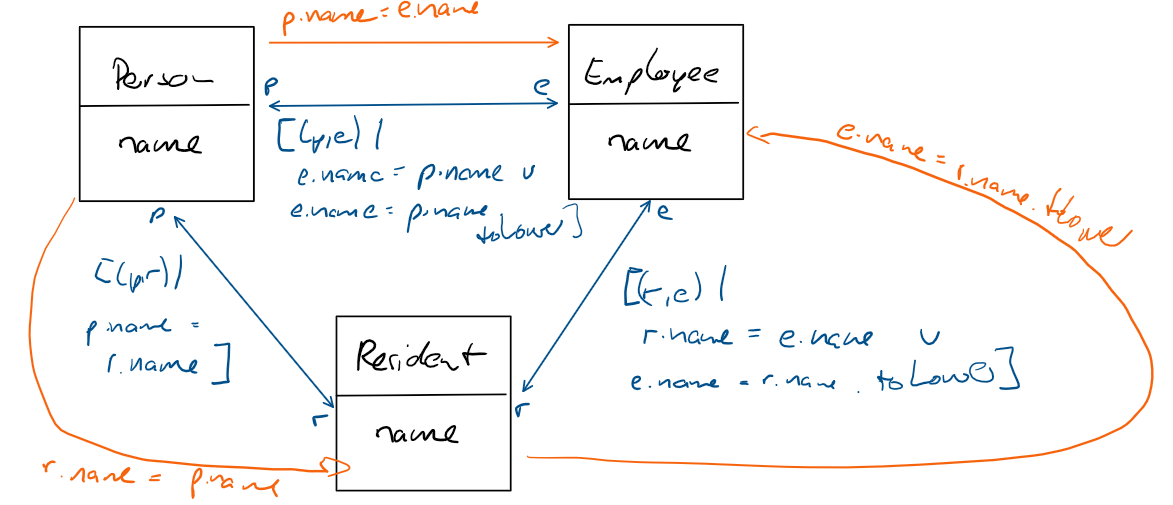
\includegraphics[width=\textwidth]{figures/correctness/orchestration/confluence.png}
    \caption[Confluence of transformations]{Counterexample for the practicality of confluence}.
    \label{fig:orchestration:confluence}
\end{figure}

\mnote{Confluence ensures that any consistent orchestration yields same result}
Confluence is an even stronger requirement than the existence of an optimal orchestration.
In literature~\cite{stevens2020BidirectionalTransformationLarge-SoSym}, confluence in a transformation network is described as the property that for given models and changes a consistent orchestration exists and that two consistent orchestrations for the same input always yield the same models.
Thus, executing transformations in any order such that the result is consistent will deliver the same result.
It is, however, easy to see that this is an impractical requirement.

\mnote{Counterexample for confluence}
In the example depicted in \autoref{fig:orchestration:confluence}, derived from the running example, three consistency relations expect for each person, employee and resident two corresponding others to exist.
They need to have the same name or, in case of the relations between persons and employees, as well as between residents and employees, the employee may have the same name in lower case.
The consistency preservation rule between persons and employees ensures that an employee with the same name exists, whereas the one between residents and employees ensures that an employee with the name in lower case exists.
Whenever a person is added, two consistent orchestrations can be distinguished.
First, the transformation between persons and employees can be executed, either followed or preceded by the one between persons and residents. Then all elements have the same name.
The models are also consistent to the relation between residents and employees, because the relation allows the names to be equal.
Second, the transformation between persons and residents can be executed, followed by the one between residents and employees.
Then the employee has the name in lower case, but still this is consistent to the relation between persons and employees.

\mnote{Confluence generally accepted as impractical}
Apart from that artificial example, such a situation can always occur if transformations have different options for elements to be consistent.
If there is not a single element that is in the overlap of consistent elements between all transformations, the result may be any of the elements in the overlap.
And the result may depend on which transformation made the first selection that fell into the overlap.
Finally, \textcite[p. 14]{stevens2020BidirectionalTransformationLarge-SoSym} also states explicitly that a network will only be confluent under very specific circumstances.

% Another intuitive notion of confluence would require that information flows together in a compatible way, i.e., the execution of a transformation does not violate consistency to other adjacent transformations.
% Formally this can be described as: A network is confluent when in every cycle of transformations t1,...tn the execution t1...ti-1 and tn,...,ti for any i leads to the same changes in the network.
% This means it does not matter in which order two transformations propagating information to the same model are executed.
% This, in consequence, means that the execution of a transformation cycles always yields models that are consistent to all transformations. Although two transformations affected the same model, consistency to the earlier executed one is not destroyed again.
% Finally, this reduces to the situation that executing each transformation once restores consistency to all transformations, which is, as we have seen, impractical.


